%! Author = Giacomo Cavalieri, Nicolò Di Domenico, Nicolas Farabegoli, Linda Vitali
%! Date = 8/5/21

% Preamble
\documentclass[final]{report}

% Packages
\usepackage[utf8]{inputenc}
\usepackage[italian]{babel}
\usepackage{graphicx}
\usepackage{listings}
\usepackage{microtype}
\usepackage{xcolor}
\usepackage{xspace}
\usepackage{enumitem}
\usepackage{csquotes}
\usepackage{booktabs}
\usepackage{float}
\usepackage[backend=biber,sorting=none]{biblatex}
\usepackage{hyperref}
\usepackage{textcomp}
\addbibresource{ecscala-report.bib}

% custom commands
\def\CC{{C\nolinebreak[4]\hspace{-.05em}\raisebox{.4ex}{\tiny\bf ++}}}
\newcommand{\eg}{\emph{e.g}\ }
\newcommand{\emailaddr}[1]{\href{mailto:#1}{\texttt{#1}}}
\newcommand{\ECS}{\textit{ECS}\xspace}
\newcommand{\Entity}{\textit{Entity}\xspace}
\newcommand{\Component}{\textit{Component}\xspace}
\newcommand{\System}{\textit{System}\xspace}
\newcommand{\entity}{\textit{entity}\xspace}
\newcommand{\component}{\textit{component}\xspace}
\newcommand{\system}{\textit{system}\xspace}
\renewcommand{\lstlistingname}{Listato}
\lstset{basicstyle=\ttfamily, showspaces=false, showstringspaces=false}
\definecolor{lightmauve}{rgb}{0.86, 0.82, 1.0}
\lstset{
    language=Scala,
    basicstyle=\footnotesize\ttfamily,
    columns=fixed,
    extendedchars=true,
    breaklines=true,
    tabsize=2,
    prebreak=\raisebox{0ex}[0ex][0ex]{},
    frame=lines,
    showtabs=false,
    showspaces=false,
    showstringspaces=false,
    keywordstyle=\color[rgb]{0.0, 0.0, 1.0},
    commentstyle=\color[rgb]{0.5,0.5,0.5},
    stringstyle=\color[rgb]{0,0.5,0},
    numbers=left,
%numberstyle=\small,
%stepnumber=1,
%numbersep=6pt,
    captionpos=b,
    escapeinside={\%*}{*)}
}

\title{ECScala - A general-purpose ECS framework}
\author{
    Giacomo Cavalieri \\
    \emailaddr{giacomo.cavalieri2@studio.unibo.it}
    \and
    Nicolò Di Domenico \\
    \emailaddr{nicolo.didomenico@studio.unibo.it}
    \and
    Nicolas Farabegoli \\
    \emailaddr{nicolas.farabegoli@studio.unibo.it}
    \and
    Linda Vitali \\
    \emailaddr{linda.vitali2@studio.unibo.it}
}

% Document
\begin{document}
    \maketitle

    \newpage

    \tableofcontents

    \newpage

    \chapter*{Introduzione}
\addcontentsline{toc}{chapter}{Introduzione}
% TODO: descrivere stato dell'arte e applicazioni di ECS
    \chapter{Processo di sviluppo}\label{ch:processo-di-sviluppo}
- Descrizione di come abbiamo usato scrum
- Descrizione come abbiamo organizzato sprint settimanali
- Descrizione di come abbiamo utilizzato github issue
- Utilizzo di file csv per tenere traccia degli sprint backlog item e product backlog
- Intero processo con PR (CI che passa -> Formattazione, Test e coverage), approvazione da tutti i membri delle PR, pair-programming, test-driven, semantic versioning.
- Definition of done
- Retrospettiva a fine sprint
    \chapter{Requisiti}\label{ch:requisiti}
Per l'individuazione dei requisiti è stato innanzitutto analizzato il pattern ECS e la terminologia adottata.
In Tabella~\ref{tab:glossario} è riportato un gloassario con i principali concetti del pattern:
\begin{table}[H]
    \begin{tabular}{p{0.15\linewidth}p{0.85\linewidth}}
        \toprule
        \textbf{World}     & Contiene più \textit{entity} e i rispettivi \textit{component}.
        Permette la registrazione di più \textit{system} che utilizza per aggiornare lo stato dei \textit{component} \\
        \textbf{View}      & Rappresenta un sottoinsieme delle \textit{entity} di un \textit{world} con i \textit{component}                                                                              \\
        \textbf{Entity}    & Contiene più \textit{entity} e i rispettivi \textit{component}                                                                                                           \\
        \textbf{Component} & Rappresenta una particolare caratteristica da modellare per una \textit{entity}                                                                                              \\
        \textbf{System}    & Aggiorna lo stato dei \textit{component} di tutte le \textit{entity} di una determinata \textit{view} secondo una logica definita dall'utilizzatore                          \\
        \bottomrule
    \end{tabular}\caption{\label{tab:glossario}Glossario dei termini del dominio.}
\end{table}

\section{Business}\label{sec:business}
L'obiettivo è quello di realizzare un framework che permetta di applicare in maniera semplice il pattern ECS\@.
I requisiti di business individuati sono:
\begin{enumerate}[label=\textbf{\ref{sec:business}.\arabic*}]
    \item \label{itm:b1} Deve essere possibile utilizzare in maniera semplice ed efficiente il pattern ECS
    \item \label{itm:b2} Il framework deve essere sufficientemente flessibile da poter realizzare simulazioni e videogiochi.
    In particolare deve essere possibile:
    \begin{enumerate}[label=\textbf{\ref{itm:b2}.\arabic*}]
        \item \label{itm:bb3} Realizzare una simulazione del moto di palle da biliardo in un tavolo da gioco
    \end{enumerate}
\end{enumerate}

\section{Utente}\label{sec:utente}
I requisiti utente sono sviluppati considerando il punto di vista dello sviluppatore che dovrà utilizzare il framework.
In particolare:
\begin{enumerate}[label=\textbf{\ref{sec:utente}.\arabic*}]
    \item \label{itm:u1} Deve essere possibile creare l'universo che contiene tutte le \textit{entità}
    \item \label{itm:u2} Deve essere possibile creare e rimuovere \textit{componenti}
    \item \label{itm:u3} Deve essere possibile creare e rimuovere \textit{entità}
    \item \label{itm:u4} Deve essere possibile creare \textit{sistemi}
    \item \label{itm:u5} Deve essere possibile utilizzare un DSL per effettuare le operazioni sopra elencate
    \item \label{itm:u6} Per l'utente è importante avere un esempio di utilizzo del framework
\end{enumerate}

\section{Funzionali}\label{sec:funzionali}
I requisiti funzionali, ricavati da quelli utente, sono:
\begin{enumerate}[label=\textbf{\ref{sec:funzionali}.\arabic*}]
    \item \label{itm:f1} Definire un \textit{mondo}
    \begin{enumerate}[label=\textbf{\ref{itm:f1}.\arabic*}]
        \item \label{itm:ff1} Definire delle \textit{viste} che selezionino alcune \textit{entità} del \textit{mondo}
        \item \label{itm:ff2} Far avanzare lo stato del \textit{mondo}, comportando l'aggiornamento delle sue \textit{entità}
    \end{enumerate}
    \item \label{itm:f2} Definire \textit{componenti}
    \item \label{itm:f3} Creare \textit{entità} all'interno di un \textit{mondo}
    \item \label{itm:f4} Rimuovere \textit{entità} dal \textit{mondo} in cui si trovano
    \item \label{itm:f5} Manipolare lo stato delle \textit{entità}
    \begin{enumerate}[label=\textbf{\ref{itm:f5}.\arabic*}]
        \item \label{itm:ff3} Aggiungere \textit{componenti} alle \textit{entità}
        \item \label{itm:ff4} Rimuovere \textit{componenti} dalle \textit{entità}
    \end{enumerate}
    \item \label{itm:f6} Creare \textit{sistemi} per manipolare i \textit{componenti} delle \textit{entità}
    \item \label{itm:f7} Registrare \textit{sistemi} nel \textit{mondo}
    \item \label{itm:f8} Fornire un DSL
    \begin{enumerate}[label=\textbf{\ref{itm:f8}.\arabic*}]
        \item \label{itm:ff5} Definire \textit{sistemi}
        \item \label{itm:ff6} Manipolare \textit{entità}
        \item \label{itm:ff7} Manipolare lo stato del \textit{mondo}
    \end{enumerate}
    \item TODO: demo %TODO: demo progetto
\end{enumerate}


\section{Non funzionali}\label{sec:non-funzionali}
Considerando gli scenari d'uso elencati al punto~\ref{itm:b2}, il sistema deve rispettare il seguente requisito:
\begin{enumerate}[label=\textbf{\ref{sec:non-funzionali}.\arabic*}]
    \item \label{itm:nf1} Aggiornare velocità e posizione di 10'000 \textit{entità} in non più di 10ms
\end{enumerate}


\section{Implementativi}\label{sec:implementativi}
\begin{enumerate}[label=\textbf{\ref{sec:implementativi}.\arabic*}]
    \item \label{itm:i1} Scala 3
    \item \label{itm:i2} Scalatest
    \item \label{itm:i3} JaCoCo per code coverage
    \item TODO %TODO citare eventuali librerie esterne
\end{enumerate}
    \chapter{Design architetturale}\label{ch:design-architetturale}
A seguito dell'analisi dei requisiti definiti nel capitolo precedente, si è realizzato il design architetturale
di massima riportato in Figura~\ref{fig:architecture}.

I principali componenti individuati sono:
\begin{itemize}
    \item \texttt{World}: permette la registrazione e rimozione di \texttt{Entity} e \texttt{System}.
    Il metodo \texttt{update} rappresenta la principale modalità di aggiornamento dello stato di un~\texttt{World}:
    infatti, comporta la modifica dei \texttt{Component} delle \texttt{Entity} secondo la logica descritta dai
    \texttt{System}.
    Inoltre, è possibile ottenere dal \texttt{World} delle \texttt{View} sulle sue \texttt{Entity}
    \item \texttt{View}: permette di selezionare le \texttt{Entity} di un \texttt{World} che abbiano tutti i
    \texttt{Component} specificati
    \item \texttt{ExcludingView}: rappresenta una specializzazione di una \texttt{View} che permette di specificare un
    ulteriore filtro andando ad indicare i \texttt{Component} che una \texttt{Entity} non deve avere per essere parte
    della \texttt{View}
    \item \texttt{System}: descrive un'operazione che viene eseguita ogni volta che viene effettuato l'\texttt{update}
    del \texttt{World} in cui è registrato
    \item \texttt{IteratingSystem}: è un wrapper di una \texttt{View} che, indicando una specifica logica di
    aggiornamento, si occupa d'iterare tutte le \texttt{Entity} selezionate aggiornandone i \texttt{Component}
    \item \texttt{ExcludingSystem}: in maniera analoga a \texttt{IteratingSystem}, è un wrapper di una
    \texttt{ExcludingView}
    \item \texttt{Entity}: permette l'aggiunta e rimozione di \texttt{Component} e il loro aggiornamento.
    Non può trovarsi in più \texttt{World} contemporaneamente
    \item \texttt{Component}: descrive una particolare caratteristica di un'\texttt{Entity} alla quale viene aggiunto.
    Non può trovarsi in più di un'\texttt{Entity} contemporaneamente;
    mantiene un riferimento all'\texttt{Entity} di appartenenza
\end{itemize}

\begin{figure}[H]
    \centering
    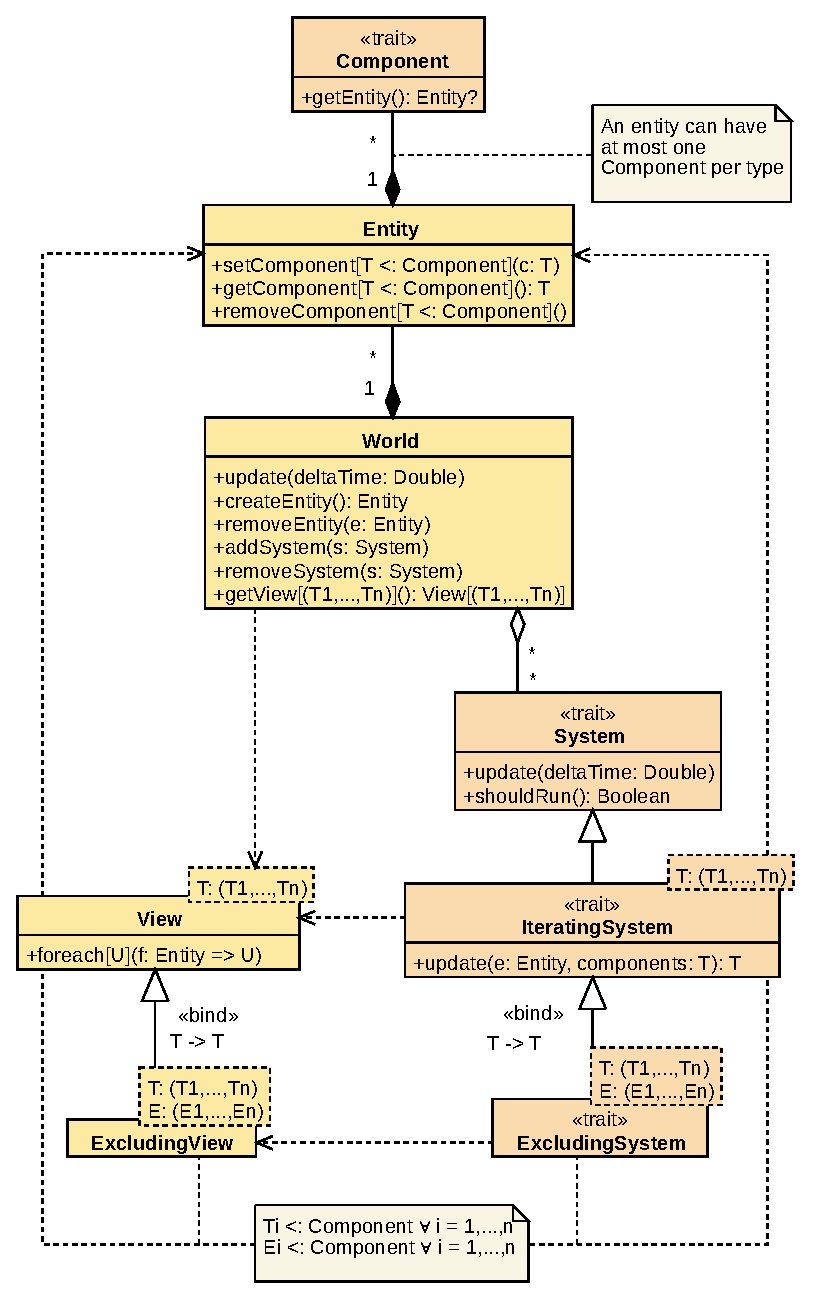
\includegraphics[width=0.95\textwidth]{./img/Architechture}
    \caption{Diagramma delle classi rappresentante l'architettura del framework.}\label{fig:architecture}
\end{figure}

In Figura~\ref{fig:sequence} è riportato il diagramma di sequenza che descrive le principali interazioni che si
verificano quando viene effettuato l'\texttt{update} di un~\texttt{World}.

\begin{figure}[H]
    \centering
    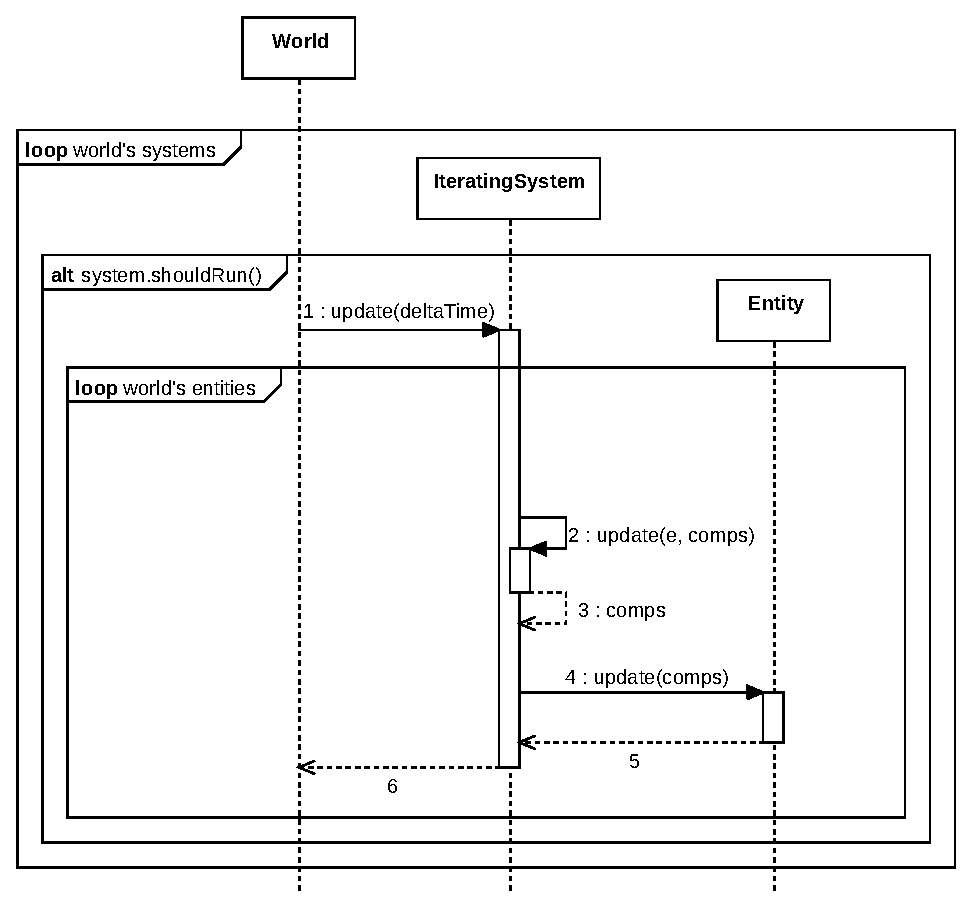
\includegraphics[width=\textwidth]{./img/Sequence}
    \caption{Diagramma di sequenza che mostra il processo di aggiornamento dei componenti nel world.}\label{fig:sequence}
\end{figure}

Una volta aggiunti i \texttt{System} al~\texttt{World}, è possibile eseguirli affinché modifichino i \texttt{Component}
su cui devono operare mediante la chiamata al metodo~\texttt{update}.
Per ogni \texttt{System} del \texttt{World} si verifica, tramite il metodo \texttt{shouldRun}, che questo possa essere
eseguito.
In caso affermativo, il sistema viene eseguito chiamandone il metodo \texttt{update}.

L'esecuzione di ogni sistema è atomica e sequenziale: ciò significa che l'ordine con cui vengono inseriti nel
mondo è significativo ai fini della computazione degli stessi e non si possono verificare race condition.

    \chapter{Design di dettaglio}\label{ch:design-di-dettaglio}
    \chapter{Implementazione}\label{ch:implementazione}
\section{Scala 3}\label{sec:scala-3}
In questa sezione vengono esaminati in che modo e dove sono stati utilizzati i nuovi costrutti di Scala 3 nel progetto.

\subsection{Impliciti}\label{subsec:impliciti}

\subsection{Macro}\label{subsec:macro}

\subsection{Context function}\label{subsec:context-function}

\subsection{Match types}\label{subsec:match-types}

\subsection{Type class}\label{subsec:type-class}

\subsection{Extension method}\label{subsec:extension-method}

\subsection{Problemi riscontrati}\label{subsec:problemi-riscontrati}
Nella libreria \texttt{scalatest} è stato riscontrato un bug nel costrutto~\texttt{shouldNot typeCheck}.
Questo costrutto consente di verificare che una espressione, definita come stringa, non passi il controllo del type
checker e di conseguenza il codice in esame non compili.
Questo controllo risulta utile nel verificare il corretto "unpacking" delle~\texttt{CList}, nello specifico si è testato
che un unpacking che contiene più elementi di quelli contenuti nella \texttt{CList} non compili;
a tal proposito si è definito il seguente test:
\lstinputlisting[label={lst:lstinputlisting22}, caption=Test per la verifica dell'unpacking delle CList.]
{./code/scalatest-bug.scala}
Nella prima asserzione si verifica l'unpacking con meno elementi di quelli nella~\texttt{CList};
nella seconda si testa lo scenario opposto, quindi l'unpacking con più elementi di quelli presenti nella~\texttt{CList}.
Per entrambi i due scenari appena descritti, la compilazione deve fallire a causa di un mismatch di tipi.
Tuttavia questo non accade poiché in entrambi i casi le espressioni vengono valutate erroneamente come valide.
Il bug è stato segnalato agli sviluppatori della libreria mediante una issue~\cite{scalatest-bug}.

Sin dalle prime fasi di sviluppo si è supportata la \textit{cross-building}~\cite{cross-building} affinché il
framework venisse compilato anche per Scala.js~\cite{scalajs}.
Questo ha generato una serie di errori all'interno dell'IDE (IntelliJ) che però non corrispondevano a errori effettivi
a livello di linguaggio;
tanto è vero che se si eseguivano i comandi di Sbt per la compilazione del progetto, quest'ultimo non sollevava alcun
tipo di errore.
A tal proposito è stata aperta una issue~\cite{intellij-issue} sul bug tracker di Jetbrains.
Per una maggiore agilità nella scrittura del codice si è quindi scelto di rimuovere la \textit{cross-building} dal
progetto.

Si segnala che, essendo il rilascio di Scala 3 relativamente recente, non è stato possibile utilizzare
le seguenti librerie per problemi di compatibilità:
\begin{itemize}
    \item Scalafix
    \item Scoverage
    \item ScalaFXML
    \item ScalaMock
\end{itemize}

\section{Benchmarks}\label{sec:benchmarks}

\section{Suddivisione del lavoro}\label{sec:suddivisione-del-lavoro}
In questa sezione viene illustrata la suddivisione del lavoro e le parti di progetto realizzate da ciascun membro del
gruppo.

\subsection{Farabegoli}\label{subsec:farabegoli}
Il contributo apportato al progetto ha toccato buona parte del core del framework e della demo.
Mi sono infine occupato della gestione del repository, della~\textit{Continuous Integration}, dei rilasci del framework
e della qualità del codice.

\subsubsection{Sviluppo collaborativo}
Spesso mi sono trovato a lavorare assieme ad altri membri del gruppo per risolvere problematiche o fornire spunti per
un migliore sviluppo del codice.
A tal proposito sono state frequenti le sessioni di lavoro in \textit{pair programming} che ci hanno consentito di
superare velocemente difficoltà nell'implementazione del codice, oltre a intercettare fin da subito potenziali bug.

\subsubsection{Component list}
La necessità di creare una tipologia di liste che contenesse al suo interno elementi di tipi diversi è nata dal fatto
che si vuole sfruttare il generico per specificare su quali~\Component devono operare i~\System (e le \View).
L'utlizzo delle liste convenzionali non è sufficiente in quanto essendo covarianti, quando si accede a un elemento della
lista, questo viene ritornato con il sopra-tipo comune della lista e non con il tipo effettivo inserito.
Si vuole quindi creare un costrutto che garantisca un livello maggiore di astrazione, mantenendo tutti gli aspetti
di type-safety noti delle liste, e che consenta anche di memorizzare elementi con tipi differenti nella stessa
collezione.
A tal proposito mi sono occupato della realizzazione delle~\texttt{CList} per rendere i~\System \textit{type-safe}
intercettando tutti gli errori dell'utente a compile-time.
La peculiarità di questa lista è data dal fatto che gli elementi in essa contenuti possono essere di tipi differenti:
questa costruzione prende il nome di~\textit{heterogeneous list}.
La costruzione delle \texttt{CList} è ispirata alla libreria \texttt{shapeless}~\cite{shapeless}.

Nel Listato~\ref{lst:lstinputlisting} viene riportata una versione semplificata d'implementazione delle \texttt{CList}.
\lstinputlisting[label={lst:lstinputlisting}, caption=Esempio di codice per implementare CList.]{code/clist.scala}

Nel contesto del framework si vuole aggiungere il vincolo tale per cui gli elementi presenti nelle \texttt{CList} siano
sottotipo di~\Component.

Oltre all'implementazione, mi sono occupato anche dello sviluppo dei test delle~\texttt{CList}: un testing approfondito
si è reputato fondamentale poiché questo costrutto rappresenta un elemento chiave dell'intero framework.
Vista la rilevante importanza del testing per questo costrutto, una parte dei test sono stati condotti assieme agli
altri membri del gruppo affinché si potessero identificare tutti i possibili casi di fallimento da intercettare.
Durante lo sviluppo dei test sopracitati si è rilevato un bug nella suite~\texttt{scalatest}; si veda la
Sezione~\ref{subsec:problemi-riscontrati} per una trattazione dettagliata del problema.

Il vantaggio offerto dalle \texttt{CList} è dato dal fatto che si può definire una lista di tipi e quindi utilizzarla
come tipo nelle funzioni che accettano un generico;
a tal proposito è stato possibile implementare \System e \View affinché accettino una \texttt{CList} nel
generico e quindi effettuino le operazioni solo sui tipi in essa definiti.

In Figura~\ref{lst:lstinputlisting2} viene mostrato un esempio di utilizzo delle \texttt{CList} nelle~\texttt{View}.
\lstinputlisting[label={lst:lstinputlisting2}, caption=Esempio di utilizzo delle CList.]{code/clist-usage.scala}

L'ordine dei tipi che definiscono una \texttt{CList} è fondamentale ai fini della computazione dei \System poiché se non
venisse rispettato si avrebbero inconsistenze di tipi che porterebbero a una condizione di errore che si vuole evitare.
Ciò consente nelle implementazioni dei \System o delle \View d'identificare a tempo di compilazione se la
\texttt{CList} che viene ritornata ha lo stesso tipo di quella dichiarata nel sistema;
se ciò non accadesse, il compilatore segnala un errore d'inconsistenza di tipi.
In questo modo garantiamo che un errato utilizzo delle \texttt{CList} venga intercettato a compile time, oltre a
preservare la semantica di utilizzo.

\subsubsection{World ed Entity}
Una delle parti che ho seguito nelle prime fasi di sviluppo è stata l'implementazione del \World e delle~\Entity.
In particolare mi sono occupato di definire l'interfaccia di entrambe le classi e di fornire una prima implementazione
di base.
Ho quindi implementato la logica delle \Entity affinché, in fase di generazione, avessero tutte un identificativo
univoco nel~\World.
Mi sono quindi occupato dello sviluppo dei test per la verifica delle classi oggetto d'implementazione.

\subsubsection{View}
Mi sono occupato di definire e implementare parzialmente la classe~\View.
Nello specifico mi sono occupato di definire l'interfaccia e fornire una prima implementazione della stessa.
Infine ho definito i test case necessari ai fini del testing della classe.
Sempre nell'ambito dello sviluppo delle~\View, Cavalieri ha sviluppato una macro per costruire la \View in modo che
operi sui componenti effettivi passati nel generico;
in questa fase ho contribuito fornendo consigli e suggerimenti per una migliore implementazione del codice.

\subsubsection{Benchmarks}
Come descritto nel requisito non funzionale~\ref{itm:nf1} si vuole ottenere un certo livello di prestazioni dal
framework.
A tal proposito ho definito una serie di benchmark che vanno a quantificare le prestazioni ottenute.
Nello specifico ho definito due benchmark: uno per le \View e uno per i~\System.
Mediante questi benchmark è stato possibile validare il requisito non funzionale sulla base di dati oggettivi.
L'aspetto di type-safety che garantiscono le \texttt{CList} è dato dal fatto che tutti i suoi componenti siano sotto tipo
di~\Component, quindi se viene costruita una~\texttt{CList} che comprenda un tipo che non è sotto tipo di~\Component,
allora l'errore viene intercettato a compile-time.

\subsection{Di Domenico}\label{subsec:nicolò-di-domenico}

Il mio ruolo nel progetto è stato principalmente quello d'implementare le \texttt{View} e i \texttt{System}, nonché
applicare ove necessario eventuali ottimizzazioni per rispettare il requisito non funzionale \ref{itm:nf1}.

\subsubsection{View}

Essendo le \texttt{View} ed \texttt{ExcludingView} progettate come indicato in Figura~TODO, si è rivelato utile costruire un
iteratore astratto che permettesse di fattorizzare tutto il codice comune.
In particolare si noti come la \texttt{ExcludingView} itera su un sottoinsieme delle entità ritornare dalla stessa
\texttt{View}, che invece non esprime vincoli di esclusione di componenti.
Per questo motivo è stato creato il \texttt{BaseViewIterator}, che si occupa di recuperare dal
\texttt{ComponentsContainer} tutte le mappe che associano ciascuna entità all'istanza (se presente) del componente di
ciascun tipo.
Infine, partendo da tali mappe, si occupa di testare l'appartenenza alla view di ciascuna entità e, in caso affermativo,
estrarne tutti i componenti richiesti.

Una semplice ottimizzazione utilizzata per rendere più veloce l'iterazione di una \texttt{View} consiste nell'individuare
la mappa di componenti con meno elementi;
una volta trovata, si iterano tutte le entità contenute al suo interno e per ognuna si controlla che sia presente in tutte
le altre mappe.
In caso affermativo, si procede all'estrazione di tutti i suoi componenti richiesti.

\subsubsection{System}

Un \texttt{System} è un blocco di codice che può essere aggiunto al \texttt{World} e viene chiamato a ogni aggiornamento
di stato della simulazione.
Ogni \texttt{System} ha due metodi:
\begin{itemize}
    \item \texttt{shouldRun}: metodo booleano che indica se il \texttt{System} dev'essere eseguito
    \item \texttt{update}: metodo che contiene il codice arbitrario da eseguire
\end{itemize}

Su di esso sono stati costruiti \texttt{IteratingSystem} ed \texttt{ExcludingSystem}, due wrapper type-safe
rispettivamente per \texttt{View} ed \texttt{ExcludingView}.
Questi due sistemi definiscono i seguenti metodi:
\begin{itemize}
    \item \texttt{shouldRun}: metodo booleano che indica se l'\texttt{IteratingSystem} dev'essere eseguito
    \item \texttt{before}: metodo eseguito prima di iterare su tutte le entità con i componenti richiesti
    \item \texttt{update}: metodo eseguito per ciascuna entità contenente le operazioni da effettuare sui suoi
    componenti richiesti
    \item \texttt{after}: metodo eseguito dopo aver iterato su tutte le entità con i componenti richiesti
\end{itemize}

Il metodo \texttt{update} deve ritornare una \texttt{CList} dei nuovi componenti;
grazie all'utilizzo delle \texttt{CList} (descritte in dettaglio in TODO) verrà verificato a tempo di compilazione che i
nuovi componenti abbiano lo stesso tipo di quelli su cui opera il sistema.
Per permettere la cancellazione di alcuni dei componenti, è stato implementato un \textit{match type} chiamato
\texttt{Deletable[L~<:~CList]}, come mostrato nel Listato~\ref{lst:deletable};
il suo scopo è quello di permettere l'inserimento in ogni posizione della \texttt{CList} un componente speciale chiamato
\texttt{Deleted}: in tal caso il componente in quella posizione sarà cancellato.

\lstinputlisting[label={lst:deletable}, caption=Implementazione del tipo \texttt{Deletable[L~<:~CList]}]{./code/deletable.scala}

L'\texttt{ExcludingSystem} è completamente analogo all'\texttt{IteratingSystem}, in quanto cambia solo la \texttt{View}
usata per ottenere le entità sulle quali iterare.
    \chapter{Retrospettiva}\label{ch:retrospettiva}

    \printbibliography

\end{document}